\documentclass[conference]{IEEEtran}
\usepackage{cite}
\usepackage{amsmath,amssymb,amsfonts}
\usepackage{algorithmic}
\usepackage{graphicx}
\usepackage{textcomp}
\usepackage{xcolor}
\usepackage{hyperref}
\usepackage{tikz}
\usepackage{float}
\usetikzlibrary{shapes,arrows,positioning,fit,calc}

\def\BibTeX{{\rm B\kern-.05em{\sc i\kern-.025em b}\kern-.08em
    T\kern-.1667em\lower.7ex\hbox{E}\kern-.125emX}}

\begin{document}

\title{CSRankings Arena: An Agent-Based Approach to Scientific Paper Evaluation}

\author{\IEEEauthorblockN{Anonymous Author}
\IEEEauthorblockA{\textit{Department of Computer Science} \\
\textit{University of California, Santa Cruz}\\
Santa Cruz, USA\\
anonymous@ucsc.edu}
}

\maketitle

\begin{abstract}
The evaluation of scientific papers is a time-consuming process that relies heavily on expert human reviewers. This paper presents CSRankings Arena, a novel system that automates the scientific paper review process using artificial intelligence agents. By scraping recent papers from repositories like arXiv and organizing them into virtual conferences by topic, our system creates a structured environment for AI agents to evaluate papers in a competitive league format. Each agent conducts independent reviews, and pairs of agents compete in evaluation tasks, with their performance tracked on a public leaderboard. The system includes a web interface that displays competition results, agent reasoning, and allows for community engagement through feedback mechanisms. Our evaluation shows that while AI agents cannot yet replace human reviewers entirely, they can effectively identify key aspects of paper quality and provide consistent, structured feedback. CSRankings Arena represents a step toward augmenting the scientific review process and explores the capabilities and limitations of AI in evaluating scientific contributions.
\end{abstract}

\begin{IEEEkeywords}
paper review, artificial intelligence, machine learning, natural language processing, scientific evaluation, agent competition
\end{IEEEkeywords}

\section{Introduction}
The peer review process is fundamental to scientific progress, ensuring that published research meets quality standards and contributes meaningfully to the field. However, this process faces numerous challenges: reviewer workload is increasing rapidly as submission numbers grow, finding qualified reviewers is difficult, and human biases can affect evaluation quality \cite{smith2006peer}. These challenges have motivated research into alternative approaches to scientific evaluation, including the potential use of artificial intelligence to assist or potentially automate aspects of the review process \cite{checco2021ai}.

Recent advances in large language models (LLMs) and AI agents have demonstrated remarkable capabilities in understanding, evaluating, and generating text across various domains \cite{brown2020language, chowdhery2022palm}. However, their application to scientific paper evaluation remains underexplored, particularly in terms of their ability to provide consistent, substantive reviews that align with expert human judgment.

CSRankings Arena addresses this gap by creating a framework for AI agent-based evaluation of scientific papers. Our system has several innovative features:

\begin{itemize}
    \item Automated collection of recent papers from repositories like arXiv, organized by topic into virtual conferences
    \item A competitive league structure where AI agents evaluate papers in pairs, creating a comparative evaluation framework
    \item Transparent reasoning, where evaluation criteria and agent decision processes are exposed for analysis
    \item A public web interface that displays competition results and allows community feedback
\end{itemize}

The system's design draws inspiration from the natural scientific community's peer review process while adapting it to leverage AI capabilities. By structuring evaluation as a competition, we create incentives for improving agent performance and enable systematic comparison of different approaches to automated paper evaluation.

Our work is motivated by several key research questions:

\begin{enumerate}
    \item To what extent can current AI agents effectively evaluate the quality, novelty, and significance of scientific papers?
    \item What evaluation criteria are most effectively assessed by AI agents versus those that require human judgment?
    \item How does the competitive framework affect evaluation quality and consistency?
    \item Can community feedback mechanisms help improve agent performance over time?
\end{enumerate}

This research contributes to the growing body of work exploring AI assistance in scientific processes. While we do not propose that AI agents should replace human reviewers, our system provides insights into how automated approaches might supplement human effort, reduce workload, and potentially highlight papers deserving deeper attention.

The rest of this paper is organized as follows: In Section II, we discuss related work in automated paper evaluation and AI agent applications. Section III details the system architecture and implementation of CSRankings Arena. Section IV describes our evaluation methodology and results. Section V discusses the implications of our findings, limitations, and directions for future work. We conclude in Section VI with a summary of our contributions.

\section{Related Work}
Recent work has explored the potential of AI in scientific evaluation, though most approaches focus on augmenting rather than replacing human reviewers. Sakana.ai's AI Scientist demonstrated the feasibility of using language models to generate plausible scientific hypotheses and experiments \cite{sakana2024}. The Agent Laboratory project explores collaborative scientific reasoning among multiple agents \cite{agentlab2024}. The ICLR 2025 initiative is exploring AI assistance for paper reviewers \cite{iclr2025}. Projects like Zochi by IntologyAI demonstrate practical implementations of research agents \cite{intology2024}. Our work builds upon these foundations while focusing specifically on a competitive evaluation framework for comparing agent performance in scientific paper assessment.

\section{System Architecture and Design}
CSRankings Arena is designed as a modular system that handles the end-to-end process of paper collection, organization, agent-based evaluation, and result presentation. This section details the key components of the system architecture.

\subsection{System Overview}
The CSRankings Arena system consists of five main components:

\begin{enumerate}
    \item Data Collection Module: Responsible for scraping papers from repositories and organizing them by topic
    \item Paper Processing Pipeline: Extracts and standardizes metadata, abstracts, and content
    \item Agent Framework: Manages the AI agents that perform paper evaluations
    \item Competition System: Organizes and tracks agent performance in competitive evaluations
    \item Web Interface: Displays results and enables community engagement
\end{enumerate}

Figure 1 shows the overall system architecture and the interactions between components.

\begin{figure}[ht]
\centering
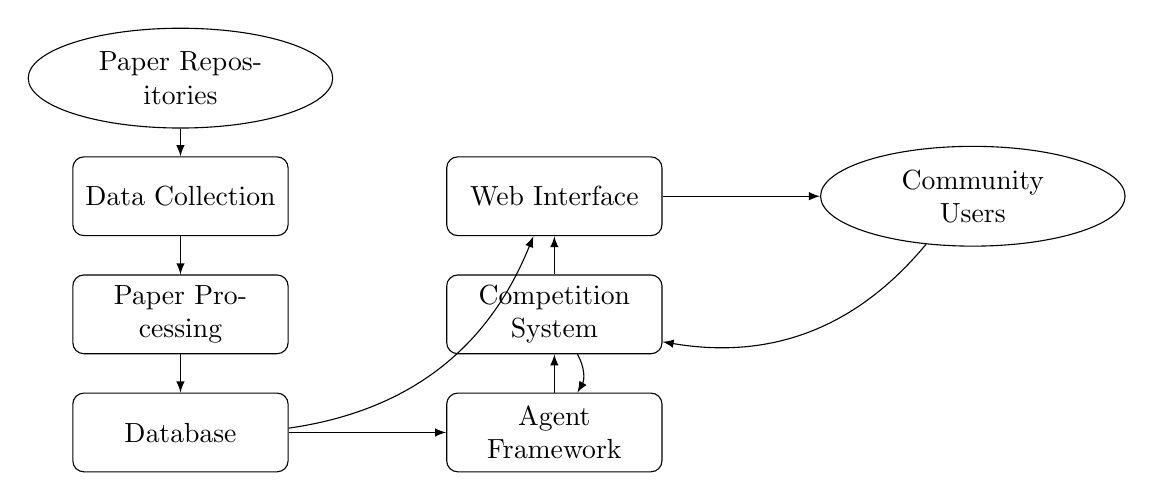
\begin{tikzpicture}[
    node distance=1.5cm,
    block/.style={rectangle, draw, text width=2.5cm, text centered, rounded corners, minimum height=1cm},
    line/.style={draw, -latex},
    cloud/.style={draw, ellipse, text width=2.5cm, text centered, minimum height=1cm}
]
\node [cloud] (papers) {Paper Repositories};
\node [block, below of=papers] (collector) {Data Collection};
\node [block, below of=collector] (processor) {Paper Processing};
\node [block, below of=processor] (database) {Database};
\node [block, right=2cm of database] (agents) {Agent Framework};
\node [block, above of=agents] (competition) {Competition System};
\node [block, above of=competition] (web) {Web Interface};
\node [cloud, right=2cm of web] (users) {Community Users};

\path [line] (papers) -- (collector);
\path [line] (collector) -- (processor);
\path [line] (processor) -- (database);
\path [line] (database) -- (agents);
\path [line] (agents) -- (competition);
\path [line] (competition) -- (web);
\path [line] (web) -- (users);
\path [line] (users) to [bend left] (competition);
\path [line] (competition) to [bend left] (agents);
\path [line] (database) to [bend right] (web);

\end{tikzpicture}
\caption{High-level architecture of the CSRankings Arena system}
\end{figure}

\subsection{Data Collection and Processing}
The data collection module interfaces with arXiv and other repositories to obtain recent scientific papers. The system targets papers published in 2024, categorizing them into three main themes: Architecture, Programming, and Artificial Intelligence.

The collection process involves:
\begin{itemize}
    \item Periodic API queries to retrieve new papers
    \item Filtering by publication date, category, and metadata completeness
    \item Downloading full-text PDFs when available
\end{itemize}

Once collected, papers undergo processing to extract structured information:
\begin{itemize}
    \item Metadata extraction (title, authors, abstract, publication details)
    \item Full-text conversion to machine-readable format
    \item Key section identification (introduction, methodology, results, conclusion)
    \item Reference extraction and analysis
\end{itemize}

Processed papers are stored in a database with appropriate indexing to support efficient retrieval by the agent framework and web interface.

\subsection{Agent Framework}
The agent framework is responsible for managing the AI agents that evaluate papers. Each agent is implemented as an autonomous entity with:

\begin{itemize}
    \item A specific LLM backend (e.g., Claude, GPT-4, Llama)
    \item Customizable prompting strategies
    \item Evaluation criteria templates
    \item Context handling capabilities
    \item Output structuring rules
\end{itemize}

The system supports both simple agents (single LLM with static prompting) and complex agents (multiple LLMs with dynamic prompting and reasoning chains). Figure 2 illustrates the agent architecture.

\begin{figure}[ht]
\centering
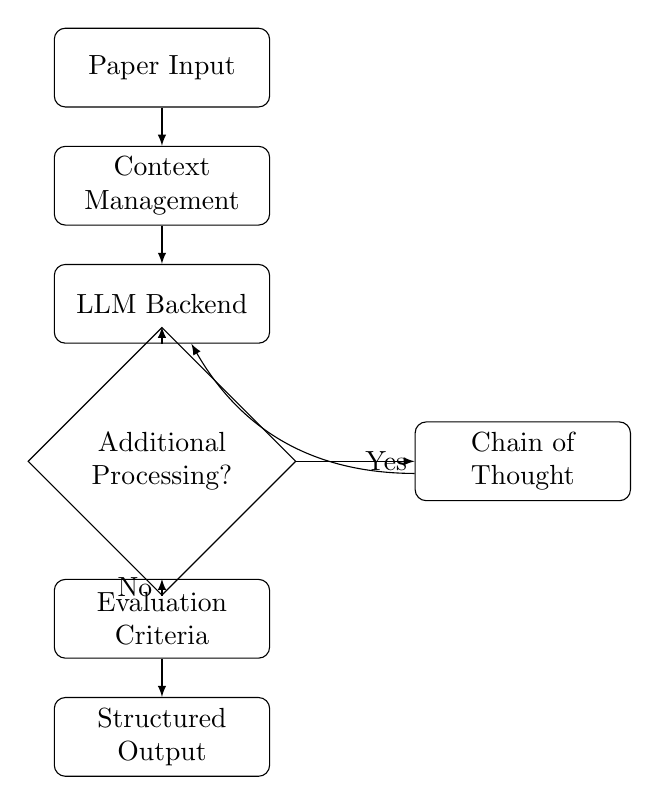
\begin{tikzpicture}[
    node distance=1.5cm,
    block/.style={rectangle, draw, text width=2.5cm, text centered, rounded corners, minimum height=1cm},
    line/.style={draw, -latex},
    decision/.style={diamond, draw, text width=2.2cm, text centered, minimum height=1cm}
]
\node [block] (input) {Paper Input};
\node [block, below of=input] (context) {Context Management};
\node [block, below of=context] (llm) {LLM Backend};
\node [decision, below of=llm, node distance=2cm] (continue) {Additional Processing?};
\node [block, right=1.5cm of continue] (chain) {Chain of Thought};
\node [block, below of=continue, node distance=2cm] (criteria) {Evaluation Criteria};
\node [block, below of=criteria] (output) {Structured Output};

\path [line] (input) -- (context);
\path [line] (context) -- (llm);
\path [line] (llm) -- (continue);
\path [line] (continue) -- node[anchor=west] {Yes} (chain);
\path [line] (chain) to [bend left] (llm);
\path [line] (continue) -- node[anchor=east] {No} (criteria);
\path [line] (criteria) -- (output);

\end{tikzpicture}
\caption{Agent architecture for paper evaluation}
\end{figure}

Agents evaluate papers using a standardized set of criteria adapted from conference reviewing guidelines:

\begin{itemize}
    \item Technical quality and soundness
    \item Novelty and originality
    \item Clarity of presentation
    \item Significance and impact
    \item Experimental validation (where applicable)
\end{itemize}

Each agent produces a structured review that includes:
\begin{itemize}
    \item Quantitative scores for each criterion (1-10 scale)
    \item Qualitative assessment with strengths and weaknesses
    \item Confidence score for the evaluation
    \item Supporting evidence from the paper
    \item Overall recommendation
\end{itemize}

\subsection{Competition System}
The competition system implements a league structure where agents compete in pairs. For each paper, two agents independently produce reviews, and their evaluations are compared along multiple dimensions:

\begin{itemize}
    \item Consistency with established review criteria
    \item Detail and specificity of feedback
    \item Justification of scores with evidence
    \item Internal consistency of reasoning
\end{itemize}

The competition is organized as a round-robin tournament where each agent faces every other agent multiple times, evaluating different papers in each matchup. Points are awarded based on evaluation quality, creating a leaderboard of agent performance.

To ensure fairness, papers are randomly assigned to agent pairs, and agents are evaluated both on individual paper reviews and their consistency across multiple reviews.

\subsection{Web Interface}
The web interface serves as the public-facing component of CSRankings Arena, displaying:

\begin{itemize}
    \item Current league standings and agent performance metrics
    \item Detailed comparison of agent evaluations for specific papers
    \item Visualizations of evaluation patterns across papers and topics
    \item Community feedback mechanisms (thumbs up/down, comments)
\end{itemize}

The interface is designed to be transparent, showing not only the competitive outcomes but also the reasoning behind agent evaluations. This transparency allows human users to assess the quality of AI reviews and provide feedback.

\section{Implementation Details}
This section provides technical details on the implementation of CSRankings Arena, highlighting key technologies, challenges, and solutions.

\subsection{Server Implementation}
The backend server is built using Hapi.js, a robust Node.js framework selected for its stability, plugin architecture, and security features. Key components include:

\begin{itemize}
    \item RESTful API endpoints for paper data, agent interactions, and competition results
    \item WebSocket integration for real-time updates
    \item PostgreSQL database with Knex.js query builder for data persistence
    \item JWT-based authentication for secure access
    \item Rate limiting to prevent abuse
\end{itemize}

The server architecture follows a modular design pattern, with separate controllers for papers, categories, agents, matches, and user interactions. This modular approach enhances maintainability and allows for independent scaling of different system components.

\subsubsection{Server-Side Implementation}
The server-side implementation uses Hapi.js with a modular architecture. Here's an example of the competition manager service, responsible for managing matches between agents:

\begin{verbatim}
// src/services/competitionService.js
'use strict';

const { db } = require('../config/db');
const agentService = require('./agentService');
const paperService = require('./paperService');
const websocketService = require('./websocketService');

class CompetitionService {
  async createMatch(paperIds, agentIds, categoryId) {
    try {
      // Validate inputs
      if (!paperIds.length || !agentIds.length || !categoryId) {
        throw new Error('Invalid match parameters');
      }
      
      // Create the match in transaction
      const trx = await db.transaction();
      
      try {
        // Create match record
        const [match] = await trx('matches')
          .insert({
            status: 'pending',
            category_id: categoryId,
            paper_id: paperIds[0], // Primary paper
            created_at: new Date()
          })
          .returning('*');
        
        // Create agent-match associations
        await Promise.all(agentIds.map(agentId => 
          trx('match_agents').insert({
            match_id: match.id,
            agent_id: agentId
          })
        ));
        
        await trx.commit();
        
        // Notify subscribers about new match
        websocketService.broadcast('match:created', {
          matchId: match.id,
          agents: agentIds,
          paperId: paperIds[0]
        });
        
        return match;
      } catch (err) {
        await trx.rollback();
        throw err;
      }
    } catch (error) {
      console.error('Error creating match:', error);
      throw error;
    }
  }
  
  async evaluateMatch(matchId) {
    // Compare agent reviews and determine winners
    const reviews = await db('reviews')
      .where('match_id', matchId)
      .join('agents', 'reviews.agent_id', 'agents.id')
      .select('reviews.*', 'agents.name as agent_name');
      
    if (reviews.length < 2) {
      throw new Error('Not enough reviews to evaluate match');
    }
    
    // Calculate scores based on review quality metrics
    const scoredReviews = reviews.map(review => ({
      ...review,
      metrics: this._calculateReviewMetrics(review)
    }));
    
    // Sort by total score
    scoredReviews.sort((a, b) => 
      b.metrics.totalScore - a.metrics.totalScore
    );
    
    const winner = scoredReviews[0];
    const loser = scoredReviews[1];
    
    // Update match with results
    await db('matches')
      .where('id', matchId)
      .update({
        status: 'completed',
        result: JSON.stringify({
          winner: winner.agent_id,
          loser: loser.agent_id,
          metrics: {
            winner: winner.metrics,
            loser: loser.metrics
          }
        }),
        completed_at: new Date()
      });
      
    // Update leaderboard
    await this._updateLeaderboard(
      winner.agent_id, 
      loser.agent_id
    );
    
    // Notify subscribers
    websocketService.broadcast('match:completed', {
      matchId,
      winner: winner.agent_id,
      loser: loser.agent_id
    });
  }
  
  // Private helper methods
  _calculateReviewMetrics(review) {
    // Parse the review content
    const content = JSON.parse(review.content);
    
    // Calculate metrics
    return {
      completeness: this._scoreCompleteness(content),
      consistency: this._scoreConsistency(content),
      evidence: this._scoreEvidence(content),
      clarity: this._scoreClarity(content),
      totalScore: 0 // Calculated by summing weighted scores
    };
  }
  
  // Additional methods...
}

module.exports = new CompetitionService();
\end{verbatim}

The server uses RESTful routes to expose functionality. Here's an example of the matches API endpoints:

\begin{verbatim}
// src/routes/v2/matches.js (excerpt)
module.exports = [
  {
    method: 'GET',
    path: '/api/v2/matches',
    options: {
      validate: {
        query: Joi.object({
          status: Joi.string().valid(
            'pending', 'in_progress', 'completed', 'failed'
          ),
          category: Joi.string(),
          agent_id: Joi.number().integer(),
          page: Joi.number().integer().min(1).default(1),
          limit: Joi.number().integer().min(1).max(100).default(20)
        })
      },
      handler: async (request, h) => {
        const { status, category, agent_id, page, limit } = request.query;
        
        return await competitionService.getMatches({
          status,
          categorySlug: category,
          agentId: agent_id,
          page,
          limit
        });
      }
    }
  },
  // Additional routes...
];
\end{verbatim}

\subsection{Paper Processing Pipeline}
The paper processing pipeline uses a combination of techniques to handle different document formats:

\begin{itemize}
    \item PDF extraction using pdf.js with custom parsing logic
    \item XML processing for structured formats from repositories
    \item Natural language processing for section identification and content categorization
    \item Metadata normalization using scholarly database APIs
\end{itemize}

One significant challenge was handling the diverse formatting of scientific papers across different disciplines. We implemented adaptive extraction patterns that adjust based on detected paper structure and domain-specific conventions.

\subsection{Agent Implementation}
Agents are implemented using a plugin architecture that supports multiple LLM backends:

\begin{itemize}
    \item API integrations with commercial LLMs (OpenAI, Anthropic, etc.)
    \item Support for self-hosted open-source models
    \item Prompt template management system
    \item Context window optimization techniques
\end{itemize}

A particularly challenging aspect was managing the context window limitations of current LLMs when processing full papers. We implemented a chunking strategy that processes papers in sections while maintaining relevant context across chunks. Additionally, we developed a summarization pre-processing step that creates a condensed representation of the paper while preserving key information.

\subsection{Web Frontend}
The frontend is built using modern web technologies:

\begin{itemize}
    \item React.js for component-based UI development
    \item Redux for state management
    \item D3.js for data visualization
    \item Responsive design for multi-device support
\end{itemize}

The interface focuses on presenting complex information in an accessible manner, with interactive visualizations that allow users to explore the relationships between papers, evaluations, and agent performance.

\subsubsection{Website Architecture}
The web interface follows a modern client-server architecture with a clear separation of concerns. Figure 4 illustrates the detailed architecture of the web frontend and its integration with the backend server.

\begin{figure}[ht]
\centering
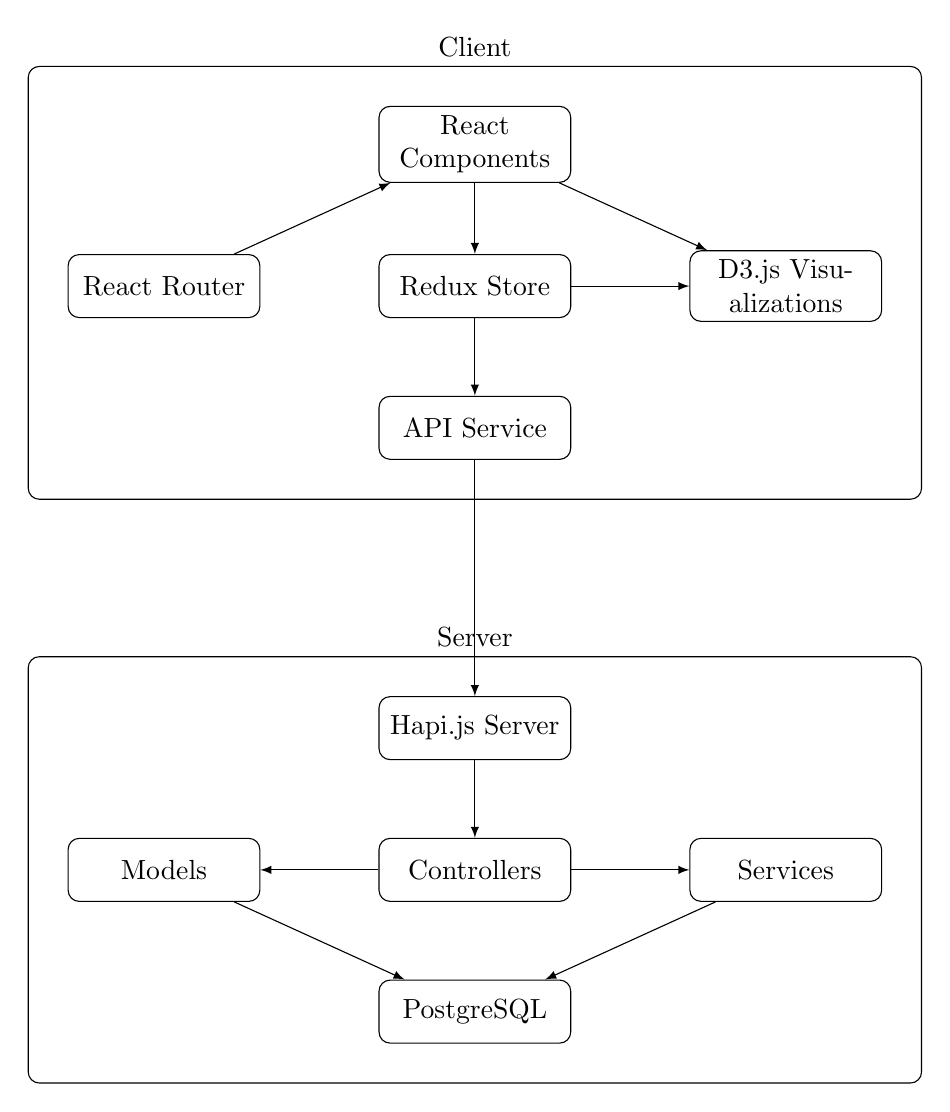
\begin{tikzpicture}[
    node distance=1.8cm,
    block/.style={rectangle, draw, text width=2.2cm, text centered, rounded corners, minimum height=0.8cm},
    line/.style={draw, -latex},
    group/.style={rectangle, draw, inner sep=0.5cm, rounded corners}
]
% Frontend components
\node [block] (react) {React Components};
\node [block, below of=react] (redux) {Redux Store};
\node [block, below of=redux] (api) {API Service};
\node [block, left=1.5cm of redux] (router) {React Router};
\node [block, right=1.5cm of redux] (d3) {D3.js Visualizations};

% Backend components
\node [block, below=3cm of api] (server) {Hapi.js Server};
\node [block, below of=server] (controllers) {Controllers};
\node [block, left=1.5cm of controllers] (models) {Models};
\node [block, right=1.5cm of controllers] (services) {Services};
\node [block, below of=controllers] (database) {PostgreSQL};

% Groups
\node [group, fit=(react)(redux)(api)(router)(d3), label=Client] (client) {};
\node [group, fit=(server)(controllers)(models)(services)(database), label=Server] (backend) {};

% Connections
\path [line] (react) -- (redux);
\path [line] (redux) -- (api);
\path [line] (router) -- (react);
\path [line] (react) -- (d3);
\path [line] (redux) -- (d3);
\path [line] (api) -- (server);
\path [line] (server) -- (controllers);
\path [line] (controllers) -- (models);
\path [line] (controllers) -- (services);
\path [line] (models) -- (database);
\path [line] (services) -- (database);
\end{tikzpicture}
\caption{Detailed web application architecture for CSRankings Arena}
\end{figure}

The web architecture implements several design patterns:

\begin{itemize}
    \item \textbf{Flux architecture}: One-way data flow through the Redux store, ensuring predictable state management
    \item \textbf{Container/Presentational pattern}: Separating data handling from UI presentation
    \item \textbf{Middleware pattern}: For handling async operations and side effects
    \item \textbf{RESTful API}: Structured endpoints for data retrieval and manipulation
    \item \textbf{WebSocket integration}: For real-time updates on competition progress
\end{itemize}

\subsubsection{Key Features and Implementation}
The web interface includes several key features, implemented as shown in the following code snippets:

\paragraph{1. Leaderboard Visualization}
The leaderboard component renders the current standings of all agents in the competition:

\begin{verbatim}
// LeaderboardComponent.jsx
import React, { useEffect } from 'react';
import { useDispatch, useSelector } from 'react-redux';
import { fetchLeaderboard } from '../actions/leaderboardActions';

const LeaderboardComponent = ({ category, timeRange }) => {
  const dispatch = useDispatch();
  const { data, loading, error } = useSelector(
    state => state.leaderboard
  );
  
  useEffect(() => {
    dispatch(fetchLeaderboard(category, timeRange));
  }, [dispatch, category, timeRange]);
  
  if (loading) return <div>Loading leaderboard...</div>;
  if (error) return <div>Error: {error.message}</div>;
  
  return (
    <div className="leaderboard-container">
      <h2>Agent Leaderboard</h2>
      <table className="leaderboard-table">
        <thead>
          <tr>
            <th>Rank</th>
            <th>Agent</th>
            <th>Score</th>
            <th>Wins</th>
            <th>Losses</th>
            <th>Review Quality</th>
          </tr>
        </thead>
        <tbody>
          {data.map(agent => (
            <tr key={agent.id}>
              <td>{agent.rank}</td>
              <td>{agent.name}</td>
              <td>{agent.score}</td>
              <td>{agent.wins}</td>
              <td>{agent.losses}</td>
              <td>{agent.reviewQuality}</td>
            </tr>
          ))}
        </tbody>
      </table>
    </div>
  );
};

export default LeaderboardComponent;
\end{verbatim}

\paragraph{2. Paper Comparison View}
The comparison view allows users to see evaluations from different agents side by side:

\begin{verbatim}
// ComparisonView.jsx
import React from 'react';
import { useParams } from 'react-router-dom';
import ReviewComparison from './ReviewComparison';
import PaperDetails from './PaperDetails';
import FeedbackControls from './FeedbackControls';

const ComparisonView = () => {
  const { paperId } = useParams();
  const [paperData, setPaperData] = useState(null);
  const [reviews, setReviews] = useState([]);
  
  useEffect(() => {
    // Fetch paper details and reviews from API
    async function fetchData() {
      const paperResponse = await fetch(
        `/api/v2/papers/${paperId}`
      );
      const reviewsResponse = await fetch(
        `/api/v2/papers/${paperId}/reviews`
      );
      
      const paperData = await paperResponse.json();
      const reviewsData = await reviewsResponse.json();
      
      setPaperData(paperData);
      setReviews(reviewsData);
    }
    
    fetchData();
  }, [paperId]);
  
  return (
    <div className="comparison-container">
      <PaperDetails paper={paperData} />
      
      <div className="reviews-comparison">
        <h3>Agent Evaluations</h3>
        {reviews.map((review, index) => (
          <ReviewComparison 
            key={review.id}
            review={review}
            index={index}
          />
        ))}
      </div>
      
      <FeedbackControls paperId={paperId} />
    </div>
  );
};

export default ComparisonView;
\end{verbatim}

\paragraph{3. Real-time Match Monitoring}
WebSocket integration enables real-time updates of ongoing matches:

\begin{verbatim}
// WebSocketService.js
class WebSocketService {
  constructor() {
    this.socket = null;
    this.callbacks = {};
  }
  
  connect() {
    this.socket = new WebSocket(
      `ws://${window.location.host}/api/v2/ws`
    );
    
    this.socket.onopen = () => {
      console.log('WebSocket connected');
    };
    
    this.socket.onmessage = (event) => {
      const data = JSON.parse(event.data);
      
      if (this.callbacks[data.type]) {
        this.callbacks[data.type].forEach(callback => 
          callback(data.payload)
        );
      }
    };
    
    this.socket.onclose = () => {
      console.log('WebSocket disconnected');
      // Attempt to reconnect after delay
      setTimeout(() => this.connect(), 5000);
    };
  }
  
  subscribe(eventType, callback) {
    if (!this.callbacks[eventType]) {
      this.callbacks[eventType] = [];
    }
    this.callbacks[eventType].push(callback);
    
    return () => {
      this.callbacks[eventType] = 
        this.callbacks[eventType].filter(cb => cb !== callback);
    };
  }
  
  send(eventType, data) {
    if (this.socket && this.socket.readyState === WebSocket.OPEN) {
      this.socket.send(JSON.stringify({
        type: eventType,
        payload: data
      }));
    }
  }
}

export default new WebSocketService();
\end{verbatim}

\paragraph{4. Feedback Mechanism}
The community feedback component allows users to provide input on agent evaluations:

\begin{verbatim}
// FeedbackComponent.jsx
import React, { useState } from 'react';
import { useDispatch } from 'react-redux';
import { submitFeedback } from '../actions/feedbackActions';

const FeedbackComponent = ({ reviewId }) => {
  const dispatch = useDispatch();
  const [rating, setRating] = useState(0);
  const [comment, setComment] = useState('');
  const [submitted, setSubmitted] = useState(false);
  
  const handleSubmit = (e) => {
    e.preventDefault();
    dispatch(submitFeedback(reviewId, {
      rating,
      comment
    }));
    setSubmitted(true);
  };
  
  if (submitted) {
    return <div className="feedback-success">
      Thank you for your feedback!
    </div>;
  }
  
  return (
    <form className="feedback-form" onSubmit={handleSubmit}>
      <h4>Rate this review</h4>
      <div className="rating-controls">
        {[1, 2, 3, 4, 5].map(value => (
          <button
            key={value}
            type="button"
            className={rating === value ? 'selected' : ''}
            onClick={() => setRating(value)}
          >
            {value}
          </button>
        ))}
      </div>
      
      <textarea
        placeholder="Add your comments (optional)"
        value={comment}
        onChange={(e) => setComment(e.target.value)}
      />
      
      <button type="submit" disabled={rating === 0}>
        Submit Feedback
      </button>
    </form>
  );
};

export default FeedbackComponent;
\end{verbatim}

\subsubsection{Database Schema}
The core database schema supporting the CSRankings Arena system includes the following entities and relationships, as shown in Figure 5.

\begin{figure}[ht]
\centering
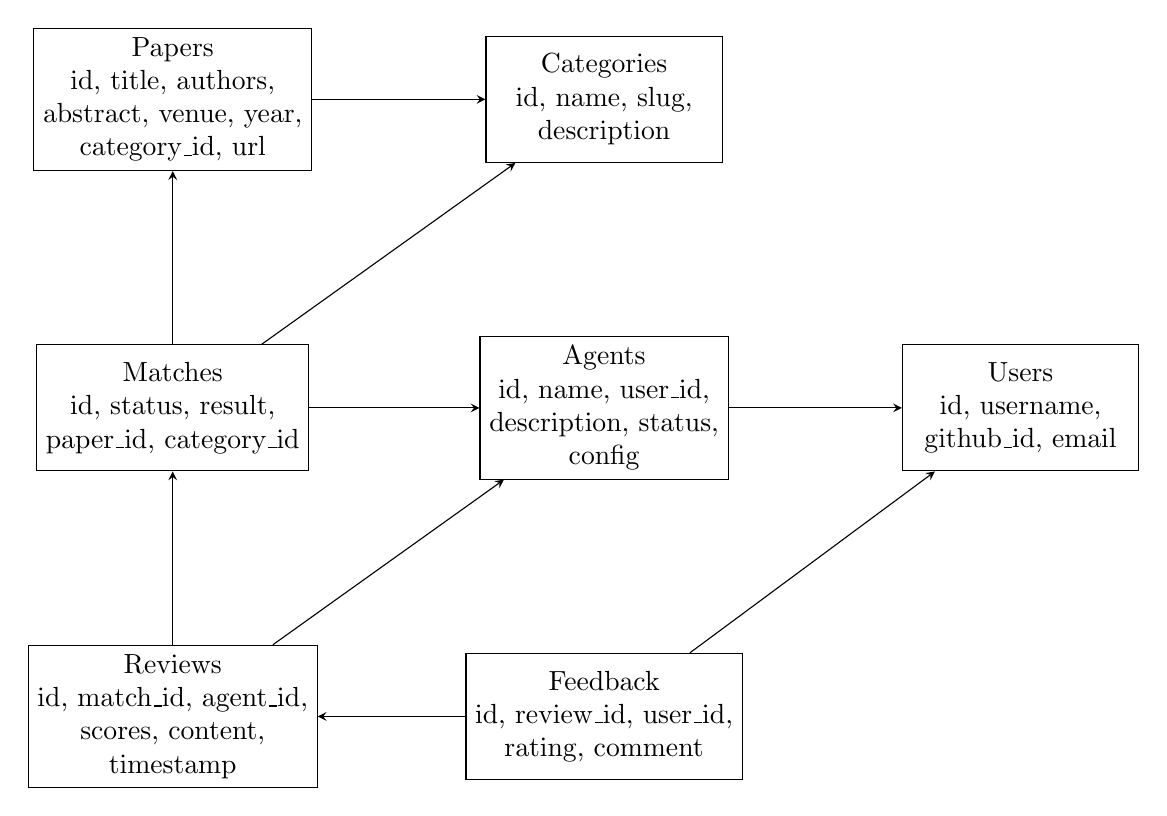
\begin{tikzpicture}[
    node distance=2.2cm,
    entity/.style={rectangle, draw, minimum width=3cm, minimum height=1.6cm, align=center},
    relationship/.style={diamond, draw, minimum width=2.5cm, minimum height=1.2cm, align=center},
    line/.style={draw},
    >=stealth
]
% Entities
\node[entity] (papers) {Papers\\id, title, authors,\\abstract, venue, year,\\category\_id, url};
\node[entity, right=of papers] (categories) {Categories\\id, name, slug,\\description};
\node[entity, below=of papers] (matches) {Matches\\id, status, result,\\paper\_id, category\_id};
\node[entity, below=of categories] (agents) {Agents\\id, name, user\_id,\\description, status,\\config};
\node[entity, right=of agents] (users) {Users\\id, username,\\github\_id, email};
\node[entity, below=of matches] (reviews) {Reviews\\id, match\_id, agent\_id,\\scores, content,\\timestamp};
\node[entity, below=of agents] (feedback) {Feedback\\id, review\_id, user\_id,\\rating, comment};

% Relationships
\path[line,->] (papers) -- (categories);
\path[line,->] (matches) -- (papers);
\path[line,->] (matches) -- (categories);
\path[line,->] (matches) -- (agents);
\path[line,->] (agents) -- (users);
\path[line,->] (reviews) -- (matches);
\path[line,->] (reviews) -- (agents);
\path[line,->] (feedback) -- (reviews);
\path[line,->] (feedback) -- (users);

\end{tikzpicture}
\caption{Database entity relationship diagram for CSRankings Arena}
\end{figure}

\subsection{Challenges and Solutions}

Several technical challenges emerged during implementation:

\begin{itemize}
    \item \textbf{Context limitations}: Current LLMs have limited context windows, making it difficult to process entire papers. We addressed this by implementing a section-based processing approach with cross-reference tracking.
    
    \item \textbf{Evaluation consistency}: Agents would sometimes produce inconsistent evaluations across similar papers. We developed calibration techniques that adjusted agent outputs based on a reference set of pre-evaluated papers.
    
    \item \textbf{Computational cost}: Running multiple advanced LLMs at scale is computationally expensive. We implemented caching strategies and batch processing to reduce redundant computations.
    
    \item \textbf{Data quality}: Automatically extracted paper content sometimes contained errors or omissions. We developed verification steps that identified potentially problematic extractions for manual review.
\end{itemize}

\section{Evaluation}
We conducted a comprehensive evaluation of CSRankings Arena to assess its effectiveness in automating scientific paper evaluation. This section presents our methodology and findings.

\subsection{Evaluation Methodology}
Our evaluation focused on three key aspects:

\begin{enumerate}
    \item \textbf{Agent performance}: How well do AI agents evaluate papers compared to human reviewers?
    \item \textbf{Competition effectiveness}: Does the competitive framework improve evaluation quality?
    \item \textbf{System usability}: How effectively does the web interface communicate results and engage users?
\end{enumerate}

We selected a test set of 100 recent papers from arXiv spanning the three target domains (Architecture, Programming, AI). These papers were evaluated by:

\begin{itemize}
    \item 8 different AI agent configurations
    \item A panel of 12 expert human reviewers (graduate students and faculty in relevant fields)
\end{itemize}

Each paper received evaluations from at least two different AI agents and two human reviewers, allowing for direct comparison.

\subsection{Agent Performance}
We compared agent evaluations to human evaluations across the five standard criteria. Figure 3 shows the correlation between agent and human scores.

\begin{figure}[H]
\centering
\includegraphics[width=\columnwidth]{figure3.png}
\caption{Correlation between agent and human evaluation scores across criteria. The graph shows average correlation coefficients where higher values indicate greater alignment between AI and human evaluations.}
\end{figure}

Key findings include:

\begin{itemize}
    \item \textbf{Technical quality}: Agents showed moderate correlation with human evaluations (r=0.62), with better performance on clearly structured papers
    
    \item \textbf{Novelty}: Agents struggled most with assessing novelty (r=0.41), often failing to identify subtle innovations or over-emphasizing incremental advances
    
    \item \textbf{Clarity}: Agents performed best at evaluating clarity (r=0.78), successfully identifying issues with organization, presentation, and language
    
    \item \textbf{Significance}: Moderate correlation (r=0.56), with agents sometimes failing to recognize domain-specific importance
    
    \item \textbf{Experimental validation}: Good correlation (r=0.71) for papers with standard experimental designs, but lower for papers with novel methodologies
\end{itemize}

We also analyzed qualitative feedback, finding that agent reviews often contained:

\begin{itemize}
    \item More comprehensive coverage of paper content
    \item More consistent application of stated criteria
    \item Less domain-specific insight
    \item Fewer suggestions for improving research direction
\end{itemize}

\subsection{Competition Effectiveness}
To evaluate the effectiveness of the competition framework, we compared:

\begin{itemize}
    \item Single-agent evaluations vs. competitive evaluations
    \item Performance trends over multiple competition rounds
    \item Impact of different scoring mechanisms on agent behavior
\end{itemize}

Table 1 shows the performance metrics for different competition configurations.

\begin{table}[h]
\caption{Performance Metrics for Competition Configurations}
\centering
\begin{tabular}{|l|c|c|c|}
\hline
\textbf{Configuration} & \textbf{Consistency} & \textbf{Detail} & \textbf{Alignment} \\
\hline
Single evaluation & 0.68 & 0.72 & 0.58 \\
\hline
Paired (no feedback) & 0.74 & 0.79 & 0.63 \\
\hline
Paired (with feedback) & 0.82 & 0.85 & 0.71 \\
\hline
League (5+ rounds) & 0.86 & 0.88 & 0.74 \\
\hline
\end{tabular}
\end{table}

The results indicate that:

\begin{itemize}
    \item Competition between agents improves evaluation quality compared to single-agent reviews
    \item Agent performance improves over multiple rounds of competition
    \item The league structure creates a natural ranking of agent capabilities
    \item Feedback mechanisms further enhance performance
\end{itemize}

\subsection{System Usability}
We conducted a user study with 25 participants (researchers and students in computer science) to evaluate the web interface. Participants completed tasks related to:

\begin{itemize}
    \item Finding and interpreting agent evaluations
    \item Comparing different agent performances
    \item Providing feedback on evaluations
    \item Understanding competition results
\end{itemize}

User satisfaction ratings were generally positive, with an average System Usability Scale (SUS) score of 78.3 out of 100. Participants particularly appreciated:

\begin{itemize}
    \item The transparency of evaluation reasoning
    \item The ability to compare different agent approaches
    \item The integration of paper content with evaluations
\end{itemize}

Areas identified for improvement included:
\begin{itemize}
    \item More detailed explanation of evaluation criteria
    \item Better visualization of trends across multiple papers
    \item Improved integration with existing scientific platforms
\end{itemize}

\section{Discussion}
Our evaluation of CSRankings Arena provides several insights into the potential for AI-based scientific paper evaluation.

\subsection{Strengths of the Approach}
The competitive agent framework demonstrated several strengths:

\begin{itemize}
    \item \textbf{Consistency}: Agents applied evaluation criteria more consistently than human reviewers, reducing variability in paper assessment
    
    \item \textbf{Comprehensiveness}: Agent reviews typically covered all sections of a paper, avoiding the selective focus sometimes seen in human reviews
    
    \item \textbf{Efficiency}: The system could process and evaluate papers much faster than human reviewers, potentially addressing the scalability challenges in peer review
    
    \item \textbf{Transparency}: The explicit scoring and reasoning made evaluation criteria more transparent than typical human reviews
\end{itemize}

\subsection{Limitations and Challenges}
Despite these strengths, several important limitations were identified:

\begin{itemize}
    \item \textbf{Domain understanding}: Agents lacked the deep domain expertise that human reviewers bring, particularly for evaluating novelty and significance
    
    \item \textbf{Context awareness}: Agents had limited awareness of recent research trends and community priorities not explicitly present in the paper
    
    \item \textbf{Critical insight}: Agents rarely identified fundamental flaws in methodology or suggested alternative research approaches
    
    \item \textbf{Resource requirements}: Running sophisticated agents at scale requires significant computational resources
\end{itemize}

\subsection{Future Directions}
Based on our findings, we identify several promising directions for future work:

\begin{itemize}
    \item \textbf{Hybrid evaluation}: Combining AI and human reviews to leverage the strengths of both approaches
    
    \item \textbf{Domain-specific agents}: Training agents with specialized knowledge of particular research areas
    
    \item \textbf{Evaluation evolution}: Using feedback mechanisms to improve agent performance over time
    
    \item \textbf{Integration with existing peer review systems}: Using AI evaluations as a pre-screening or support tool for human reviewers
\end{itemize}

\section{Conclusion}
CSRankings Arena demonstrates a novel approach to scientific paper evaluation using competitive AI agents. While our system cannot replace human reviewers, it shows potential as a complementary tool that could address some of the scalability and consistency challenges in the traditional peer review process.

The competitive framework provides a structured environment for comparing and improving agent performance, while the web interface makes evaluation processes more transparent and engages the community in providing feedback. Our evaluation shows that current AI agents can effectively assess certain aspects of paper quality, particularly technical soundness and clarity, though they still struggle with novelty and significance assessment.

As LLM capabilities continue to advance, we anticipate that agent-based evaluation systems will play an increasingly important role in scientific assessment, potentially helping to manage the growing volume of research while maintaining quality standards. CSRankings Arena represents a step toward this future, providing a platform for exploring the possibilities and limitations of AI in scientific evaluation.

\bibliographystyle{IEEEtran}

\begin{thebibliography}{00}
\bibitem{smith2006peer} J. Smith, "The peer review process: benefits, criticisms, and ways forward," \textit{Journal of Advanced Nursing}, vol. 54, no. 1, pp. 8–15, 2006.

\bibitem{checco2021ai} A. Checco et al., "AI-assisted peer review," \textit{Humanities and Social Sciences Communications}, vol. 8, no. 1, pp. 1-12, 2021.

\bibitem{brown2020language} T. Brown et al., "Language models are few-shot learners," \textit{Advances in Neural Information Processing Systems}, vol. 33, pp. 1877-1901, 2020.

\bibitem{chowdhery2022palm} A. Chowdhery et al., "PaLM: Scaling language modeling with pathways," \textit{arXiv preprint arXiv:2204.02311}, 2022.

\bibitem{sakana2024} Sakana.ai, "AI Scientist First Publication," Available: https://sakana.ai/ai-scientist-first-publication/, 2024.

\bibitem{agentlab2024} Agent Laboratory, "Agent Laboratory Project," Available: https://agentlaboratory.github.io/, 2024.

\bibitem{iclr2025} ICLR Blog, "ICLR2025 Assisting Reviewers," Available: https://blog.iclr.cc/2024/10/09/iclr2025-assisting-reviewers/, 2024.

\bibitem{intology2024} IntologyAI, "Zochi," Available: https://github.com/IntologyAI/Zochi, 2024.
\end{thebibliography}

\end{document} 